\chapter{Simulation de la Flotte IoT}
\label{chap:fleet}

\section{Présentation du dataset}

\subsection{Source des données}

Le dataset utilisé est le \textbf{IoT Communication Security Dataset}, composé de 76\,000 entrées représentant des échanges MQTT typiques d'un écosystème IoT industriel. Chaque entrée décrit les caractéristiques d'une communication : protocole, longueur du payload, durée, type d'attaque éventuel, etc.

\subsection{Distribution des classes}

\begin{table}[H]
\centering
\caption{Distribution des classes dans le dataset}
\label{tab:dataset_classes}
\begin{tabular}{lrl}
\toprule
\textbf{Classe} & \textbf{Occurrences} & \textbf{Description} \\
\midrule
Normal & 43\,200 & Trafic IoT légitime \\
DoS & 12\,600 & Inondation de connexions/messages \\
MiTM & 8\,400 & Interception et modification de paquets \\
Replay & 5\,600 & Rejeu de messages capturés \\
FalsifiedData & 3\,900 & Injection de données falsifiées \\
Scanning & 1\,400 & Scan de ports et d'infrastructure \\
Malware & 840 & Comportements de type botnet \\
\bottomrule
\end{tabular}
\end{table}

\begin{figure}[H]
  \centering
  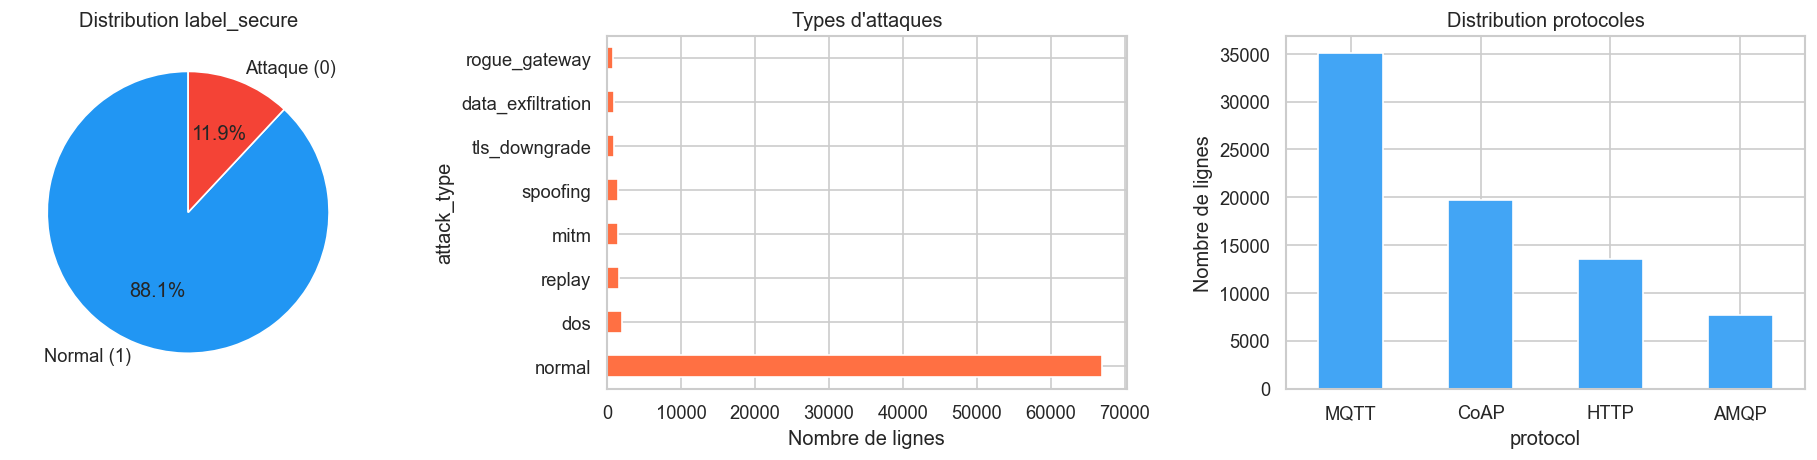
\includegraphics[width=0.7\textwidth]{figures/eda_classes_distribution.png}
  \caption{Distribution des classes dans le dataset IoT}
  \label{fig:class_dist}
\end{figure}

Le dataset présente un déséquilibre notable : la classe \textit{Normal} représente environ 57\,\% des données, tandis que la classe \textit{Malware} ne représente que 1,1\,\%. Ce déséquilibre est représentatif des conditions réelles d'un réseau IoT.

\section{Architecture du simulateur de flotte}

\subsection{Conception}

Le simulateur de flotte (\texttt{fleet\_sim.py}) est un programme Python multi-thread simulant une flotte de \textbf{50 dispositifs IoT} concurrents. Le diagramme de classes de la figure~\ref{fig:classe_fleet} détaille l'architecture logicielle du simulateur.

\begin{figure}[H]
  \centering
  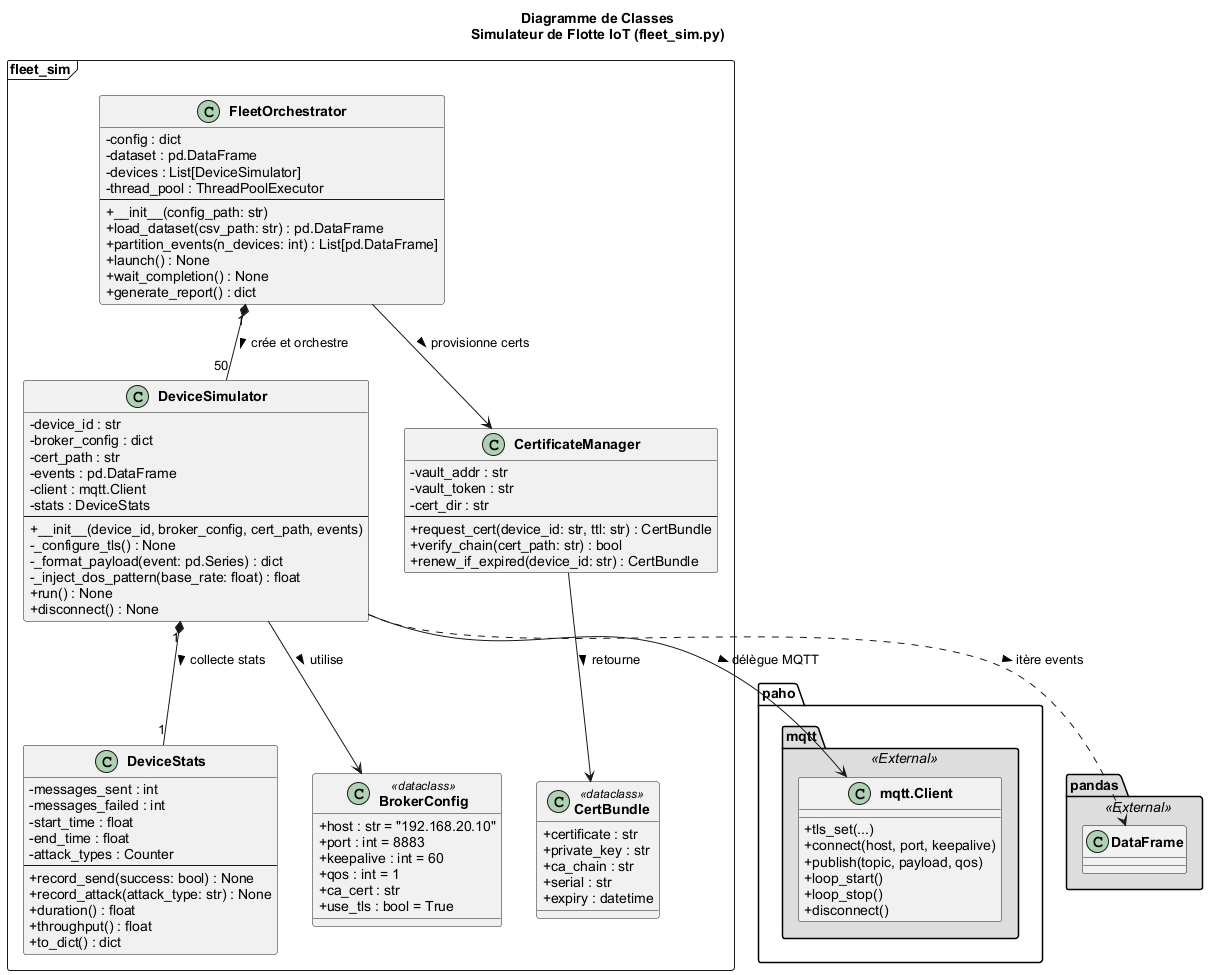
\includegraphics[width=\textwidth]{diagrams/diag-classe-fleet-sim.png}
  \caption{Diagramme de classes du simulateur de flotte IoT}
  \label{fig:classe_fleet}
\end{figure}

Chaque dispositif simulé :
\begin{itemize}
  \item Dispose d'un identifiant unique (\texttt{device-001} à \texttt{device-050}).
  \item Possède un certificat X.509 individuel émis par Vault.
  \item Publie des messages MQTT sur des topics dédiés (\texttt{iot/sensors/device-XXX/}).
  \item Reproduit fidèlement un sous-ensemble du dataset CSV (échantillonnage stratifié par classe).
\end{itemize}

\subsection{Structure logicielle}

Le simulateur est organisé autour de quatre classes principales :

\begin{description}
  \item[\texttt{FleetOrchestrator}] Classe principale qui charge le dataset, le partitionne entre les dispositifs et lance les threads concurrents via un \texttt{ThreadPoolExecutor}.
  \item[\texttt{DeviceSimulator}] Représente un dispositif IoT individuel. Configure la connexion mTLS, itère sur ses événements assignés et publie les messages MQTT.
  \item[\texttt{DeviceStats}] Collecte les statistiques de chaque dispositif : messages envoyés, erreurs, débit, types d'attaques rejoués.
  \item[\texttt{CertificateManager}] Gère l'interaction avec l'API Vault pour le provisionnement et le renouvellement des certificats.
\end{description}

Le code source complet du simulateur est fourni en Annexe~A.

\subsection{Processus de simulation}

Le diagramme d'activité de la figure~\ref{fig:fleet_activity} illustre le processus complet de simulation, depuis le chargement du dataset jusqu'à la génération du rapport final.

\begin{figure}[H]
  \centering
  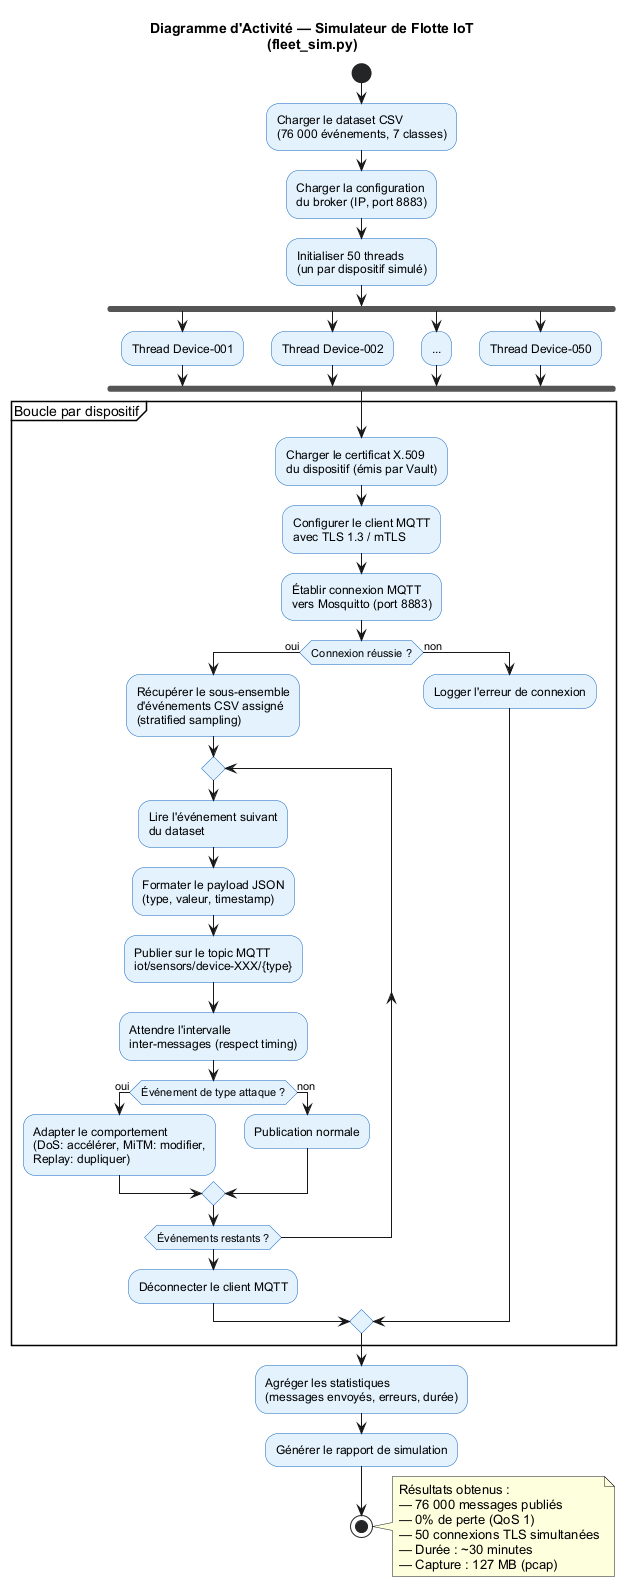
\includegraphics[width=0.7\textwidth]{diagrams/diag-fleet-activity.png}
  \caption{Diagramme d'activité du simulateur de flotte IoT}
  \label{fig:fleet_activity}
\end{figure}

\subsection{Paramètres de simulation}

\begin{table}[H]
\centering
\caption{Paramètres de la simulation}
\label{tab:sim_params}
\begin{tabular}{ll}
\toprule
\textbf{Paramètre} & \textbf{Valeur} \\
\midrule
Nombre de dispositifs & 50 \\
Durée totale de simulation & $\sim$30 minutes \\
Messages/dispositif/minute & $\sim$50 \\
Total messages publiés & 76\,000 \\
Threads concurrents & 50 \\
QoS MQTT & 1 \\
\bottomrule
\end{tabular}
\end{table}

\section{Injection des patterns d'attaque}

Les patterns d'attaque sont rejoués tels quels depuis le dataset, préservant leur temporalité et leurs caractéristiques statistiques. Pour le scénario DoS, le flux de messages est intensifié (facteur 10$\times$ par rapport au taux normal) afin de reproduire fidèlement l'inondation.

Les sept types de comportements couverts par la simulation sont :
\begin{enumerate}
  \item \textbf{Normal} -- Trafic IoT légitime (télémétrie de capteurs).
  \item \textbf{DoS} -- Connexions et publications massives vers le broker.
  \item \textbf{MiTM} -- Interception et modification des payloads.
  \item \textbf{Replay} -- Rejeu de messages précédemment capturés.
  \item \textbf{FalsifiedData} -- Injection de valeurs de capteurs falsifiées.
  \item \textbf{Scanning} -- Scan des ports et des topics du broker.
  \item \textbf{Malware} -- Comportements caractéristiques de botnets IoT.
\end{enumerate}

\section{Résultats de la simulation}

La simulation a généré avec succès l'ensemble des 76\,000 événements. La capture réseau réalisée par Suricata a confirmé la cohérence du trafic avec le dataset source.

\begin{resultbox}[Résultats de la simulation]
\begin{itemize}
  \item \textbf{76\,000 messages} publiés avec succès en mTLS.
  \item Taux de perte MQTT : \textbf{0\,\%} (QoS~1 avec retransmission).
  \item Les 50 dispositifs ont maintenu leurs connexions TLS simultanément.
  \item Fichier de capture : \texttt{results/analysis/step6/mqtt\_tls.pcap} (127~MB).
\end{itemize}
\end{resultbox}
